\section{平成31年度 専門科目}

\subsubsection{} %{問1}
\barquo{
$\R[X,Y]$を変数$X,Y$に関する実数係数の$2$変数多項式環とする。$I$を$X^2 + Y^2$で生成された$\R[X,Y]$のイデアルとする。$A = \R[X,Y]/I $とおく。このとき、以下の問に答えよ。
\begin{description}
  \item[(i)] $A$は整域であることを示せ。
  \item[(ii)] $A$の商体を$K$とおき、$A$の$K$における整閉包を$B$とおく。$A$加群としての$B$の生成系を一組与えよ。
\end{description}
}
\begin{sol} ${}$
  \begin{description}
    \item[(i)] $\R[X,Y]$はUFDなので、$X^2 + Y^2$が既約元であることを示せばよい。ハイリホーによる。可約であると仮定しよう。そうするとある実数$a,b,c,d $が存在して$X^2 + Y^2 = (aX + bY)(cX + dY)$が成り立つことになるが、その場合$ac - 1 = ad + bc = bd - 1 = 0$でなくてはならない。これは$a,b,c,d$が実数であったことに矛盾。よって$X^2 + Y^2$は既約元であり、$I \subset \R[X,Y]$は素イデアル。
    \item[(ii)] $a = Y/X$とする。$a^2 + 1 = 0$なので$a \in B$である。$B = A[a]$を示そう。それには、$A[a]$が整閉であることを示せば十分である。$\R$代数の準同形$\vp \colon \R[X,\I] \to A[a]$を$\vp(\I)=a, \vp(X)=X$で定める。これはwell-definedであり、あきらかに全射。

    また逆写像が構成できるので$\vp$は単射。よって$\vp$は同型であり、$A[a] \cong \R[X,\I] \cong \C[X]$である。$\C[X]$はPIDであり、とくにUFDでもあるから整閉である。よって$A[a]$も整閉だから$B = A[a]$が示された。よって、$B$の$A$加群としての生成系としては$\{ 1, a \}$がとれる。
  \end{description}
\end{sol}


\newpage

\subsubsection{} %{問2}
\barquo{
有限群$G$に対して、次の条件$(*)$を考える。
\begin{description}
  \item[$(*)$] 任意の正整数$n$に対して、$G$の部分群のうち、位数が$n$のものの個数は$1$以下である。
\end{description}
以下の問に答えよ。
\begin{description}
  \item[(i)] $G$は有限Abel群で$(*)$を満たすとする。このとき、$G$は巡回群であることを示せ。
  \item[(ii)] $G$は有限群で$(*)$を満たすとする。$H$を$G$の正規部分群とする。このとき、$G/H$も$(*)$を満たすことを示せ。
  \item[(iii)] $G$は有限群で$(*)$を満たすとする。このとき、$G$は巡回群であることを示せ。
\end{description}
}
\begin{proof} ${}$
  \begin{description}
    \item[(i)] ハイリホーによる。$(*)$を満たし巡回群でない$G$があったとする。有限生成Abel群の構造定理により$G$は巡回群の直和で表されており、
    \[
    G = \bigoplus_{i=1}^t \Z / m_i \Z
    \]
    なる$m_i$がある。$G$は巡回群ではないので$t \geq 2$であり、中国式剰余定理により$m_i$のなかには少なくとも一組互いに素でないものがある。その最大公約数を$e$とすると、$G$は位数$e$の部分群を少なくとも二つもつことになり矛盾。よって示せた。
    \item[(ii)] $G/H$の部分群全体$X$と、$G$の$H$を含む部分群全体$Y$の間には全単射がある。それは自然な写像$\pi \colon G \to G/H$を用いて次のようにあらわせる。
    \begin{align*}
      &X \to Y \st M \mapsto \pi^{-1}(M) \\
      &Y \to X \st K \mapsto \pi(K)
    \end{align*}
    この全単射により、位数が等しい部分群の組は位数が等しい部分群の組に送られるため、これで示すべきことがいえた。
    \item[(iii)] $G$の部分群$H$と$g \in G$に対して、$gHg^{-1} = H$でなくてはならないため、$H$は正規部分群であることに注意しておく。そうすると、$G$のSylow-$p$部分群はどの$p$についても正規部分群である。そこで$\# G$の異なる素因子を$p_1, \cdots ,p_t$として対応するSylow部分群を$H_i$とする。任意の$i,j$について交換子$[H_i,H_j]$は$H_i \cap H_j = 1$の部分集合だから、異なる$H_i$の元同士は可換である。よって積をとる写像
    $
    \prod_{i=1}^t H_i \to G
    $
    は準同形であり、全射であり、位数の考察から全単射でもある。位数が互いに素な巡回群の直積は巡回群なので、$G$ははじめから$p$群であるとしてよい。

    $\# G = p^e$とする。$e$についての帰納法で示そう。$e=1$ならば$G$はあきらかに巡回群であるから$e \geq 2$とする。よく知られているように、$p$群の中心は自明ではない。(雪江\cite{雪代1}命題4.4.3)そこで位数$p$の元$\pi \in Z(G)$が存在することがわかる。$G/\kakko{\pi}$は(ii)と帰納法の仮定により巡回群である。$G/\kakko{\pi}$の生成元の代表元として$\grs \in G$をとる。そうすると積をとる写像
    $
    \kakko{\pi} \tm \kakko{\grs} \to G
    $
    は準同形でありかつ全射で、位数の考察から全単射でもある。ゆえに$G \cong \kakko{\pi} \tm \kakko{\grs}$だから$G$はAbel群であり、したがって(i)より巡回群である。よって帰納法は回り、示すべきことが言えた。
    \end{description}
\end{proof}

\newpage


\subsubsection{} %{問3}
\barquo{
多項式$f(X) = X^4 + 6X^2 + 2 \in \Q[X]$の$\Q$上の最小分解体を$K$とおく。$K$を$\C$の部分体とみなし、$F=K \cap \R$とおく。このとき、次の問に答えよ。
\begin{description}
  \item[(i)] 拡大次数$[F : \Q]$を求めよ。
  \item[(ii)] $F/\Q$はGalois拡大であることを示せ。
\end{description}
}
\begin{proof} 以下この解答では$[\Q(\sqrt{2},\sqrt{7}): \Q ] = 4$は認めて使う。
  \begin{description}
\item[(i)] $X^4 + 6X^2 + 2$は複2次式なので因数分解ができる。
 \begin{align*}
  X^4 + 6X^2 + 2 &= (X^2 + 3)^2 - 7 \\
  &= (X^2 + 3 + \sqrt{7} )(X^2 + 3 - \sqrt{7} )
  \end{align*}
  なので、この多項式の根は
  $
  \pm i \sqrt{ 3 \pm \sqrt{7}  }
  $
  である。$\gra = i \sqrt{ 3 + \sqrt{7}  }  $, $\beta = i \sqrt{ 3 - \sqrt{7}  } $とおく。$K = \Q(\gra, \beta) = \Q(\gra, \sqrt{2})$である。
  \[
  \xymatrix{
  \Q(\sqrt{2}) \ar[r] & F \ar[r] & K \\
  \Q \ar[u] \ar[r] & \Q(\sqrt{7}) \ar[r] \ar[u] & \Q(\gra) \ar[u]
  }
  \]
  多項式$f(X)$は$p=2$に関するEisenstein多項式だから$\Q[X]$の元として既約。ゆえに$f(X)$は$\gra$の$\Q$上の最小多項式であるから$[\Q(\gra ) : \Q] = 4$である。さらに$[K:\Q] = 8$であることを示そう。$K = \Q(\gra, \sqrt{2})$なので
  $\sqrt{2} \not\in \Q(\gra)$を示せばよい。
  ハイリホーでこれを示す。仮に$\sqrt{2} \in \Q(\gra)$だったとする。このときある$b,c \in \Q(\sqrt{7})$が存在して
  \[
  \sqrt{2} = b \gra + c
  \]
  である。この式から
  \[
  \begin{cases}
    bc = 0 \\
    c^2 - (3 + \sqrt{7})b^2 = 2
  \end{cases}
  \]
を得る。$bc=0$より$b=0$または$c=0$である。$b=0$なら$\sqrt{2} \in \Q(\sqrt{7})$ということになり矛盾。$c=0$なら$N \colon \Q(\sqrt{7}) \to \Q$をノルムとすると
$
2 =  N(b)^2
$
となり$\sqrt{2} \in \Q$となって矛盾。いずれにせよ矛盾が得られたので、$\sqrt{2} \not\in \Q(\gra)$が示せた。よって$[K:\Q] = 8$である。

  一方で$\Q(\sqrt{7}, \sqrt{2}) \subset F$より$[F : \Q] \geq 4$である。かつ$F \subsetneq K$から$[F : \Q] < 8$なので、$[F : \Q] = 4$でなくてはならない。
  \item[(ii)] 包含関係があって$\Q$上の次元が同じなので$F = \Q(\sqrt{7}, \sqrt{2})$である。$\Q$は標数$0$なので完全体であり、したがって$F/\Q$は分離拡大。かつ$F$を$\Q$上生成する$\sqrt{7}$と$\sqrt{2}$の共役はすべて$F$に含まれているので、$F/\Q$はGalois拡大である。
  \end{description}
\end{proof}



\newpage


\subsubsection{} %{問4}
\barquo{
$n \geq 2$に対して、
\[
S^{n-1} = \setmid{(x_1, \cdots , x_n) \in \R^n }{x_1^2 + \cdots + x_n^2 = 1 } \quad \bbs^1 = \setmid{z \in \C}{\abs{z} = 1}
\]
とし、写像$\Phi \colon S^{n-1} \tm \bbs^1 \to \C^n$を
\[
\Phi(x_1, \cdots , x_n) = (x_1z, \cdots , x_nz)
\]
と定める。
\begin{description}
  \item[(1)] $\Phi$の像$M$が$\C^n$の実$n$次元部分多様体であることを示せ。
  \item[(2)] $n$が偶数のとき、$M$が向き付け可能であることを示せ。
\end{description}
}
\begin{sol} ${}$
  \begin{description}
    \item[(1)] $\Phi(x,z) = \Phi(y,w)$とする。すると$\forall i \; x_i z = y_i w$である。$S^{n-1}$の定義により$x_i \neq 0$なる$i$がある。よって$z/w = y_i / x_i \in \R$であるので、$z=w$または$z = -w$である。したがってず$w \in M$に対して$\# \Phi^{-1}(w) =2$であることが分かった。

    $N = S^{n-1} \tm \bbs^1$とおく。$N$に$(x,z) \sim (-x, -z)$で生成される同値関係$\sim$を定義する。このとき$\Phi(x,z) = \Phi(y,w)$と$(x,z) \sim (y,w)$は同値である。ゆえに次の図式
    \[
    \xymatrix{
    N \ar[r]^-{\Phi} \ar[d]_-{P}  & M \\
    N/ {\sim} \ar@{.>}[ru]_-{ \wt{\Phi} }
    }
    \]
    を可換にするような全単射連続写像$\wt{\Phi}$がある。$N/{\sim}$はコンパクトで、$M$はHausdorffなので$\wt{\Phi}$は同相でなければならない。したがって$M$の代わりに$N/{\sim}$が$n$次元位相多様体であることをいえばよいが、$P$が被覆写像であるためこれはあきらか。
    \item[(2)] $n$は偶数と仮定されているので$n=2k$とおける。接ベクトル束$TM$の切断$s$であって、至る所ゼロでないものの存在をいえば十分である。$\beta = (x,z) \in N$に対して
    \[
    \wt{z} = (x_2, -x_1, \cdots , x_{2k}, -x_{2k-1}, -y_2, y_1)
    \]
    と定めておき、これによりベクトル場$N \to TN \st z \mapsto (z, \wt{z})$を定める。このベクトル場は$N/{\sim}$上のベクトル場を誘導し、あきらかに至る所ゼロでない。よって示せた。
  \end{description}
\end{sol}



\newpage

\subsubsection{} %{問5}
\barquo{
$\C$の部分空間
\[
X = \setmid{1- e^{i\grt} \in \C }{0 \leq \grt < 2\pi} \cup \setmid{-1 + e^{i\grt} \in \C}{0 \leq \grt < 2\pi }
\]
を考える。整数$p,q$に対して、写像$f \colon X \to X$を
\begin{align*}
  f(1- e^{i\grt}) &= -1 + e^{ip\grt} \\
    f(-1 + e^{i\grt}) &= 1 - e^{iq\grt}
\end{align*}
で定め、$X \tm [0,1]$に
\[
(x,0) \sim (f(x),1)
\]
($x \in X$)で生成される同値関係$\sim$を与える。商空間$Y = (X \tm [0,1])/ {\sim}$の整数係数ホモロジー群を計算せよ。
}
\begin{sol}

セル複体を使ってホモロジーを求めよう。空間$Y$を直接書くことは難しいが、次のようなものを想像することはできる。

\begin{center}
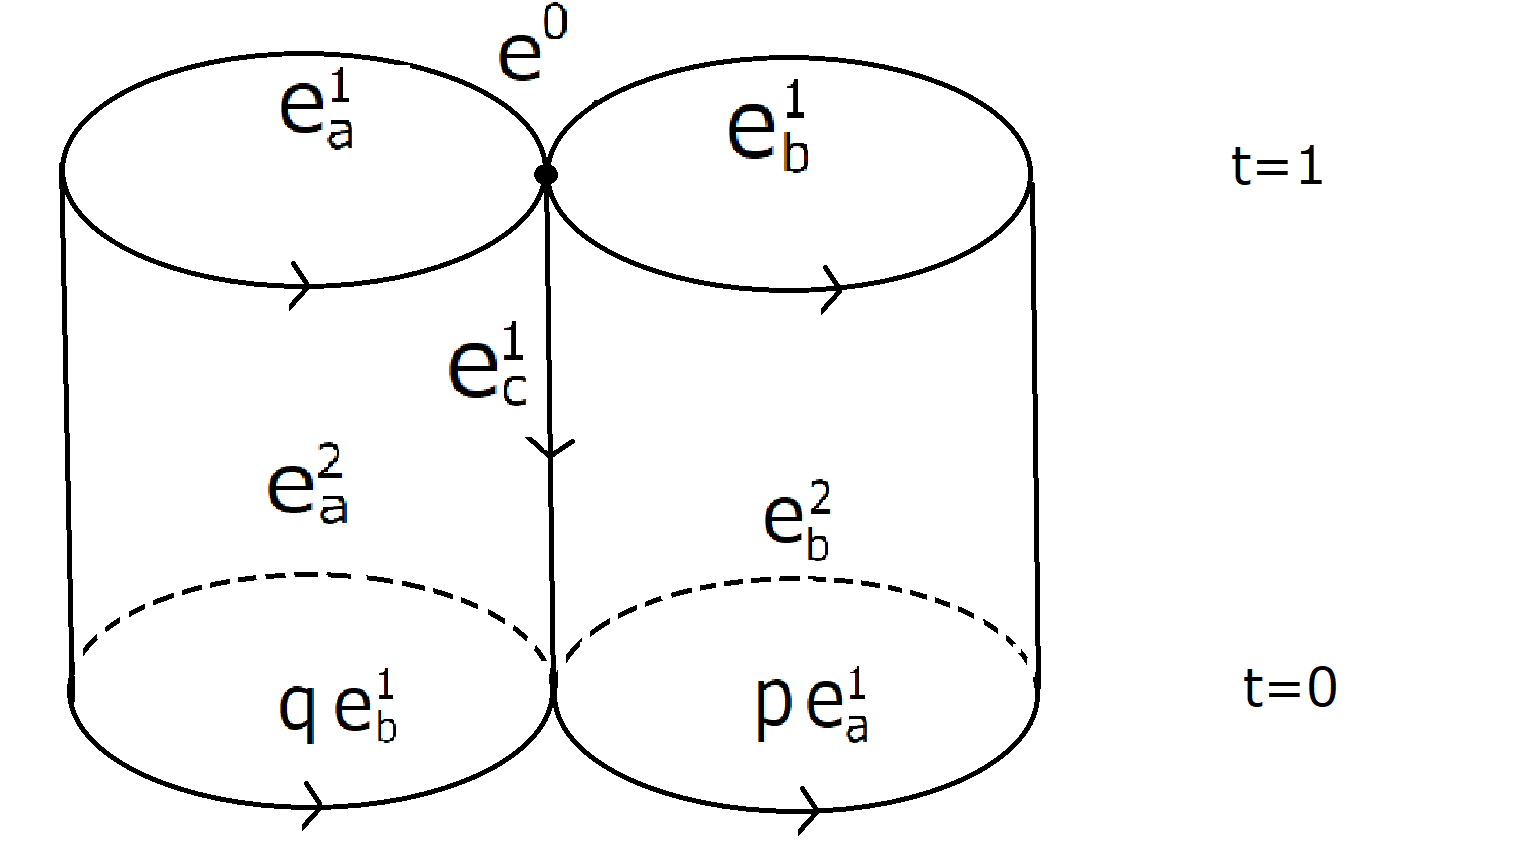
\includegraphics[width=5cm]{H31expert05_01.png}
\end{center}

この対になった円筒は、$X \tm I$および$Y$を表している。上下の円盤に見える部分は円周であり、ちくわを2つくっつけたような形をしている。側面も輪郭しか書かれていないが、面になっている。垂直方向が$I$成分を表しており、上が$t=1$で下が$t=0$であるものとしよう。また右を実軸のプラス方向、奥を虚軸のプラス方向とする。上部にある点は原点を表す。図に$e$と書かれているのはセルである。それぞれ具体的には次のように与えられる。
\begin{align*}
  e^0 &= (0,1) \\
  e^1_a &= \setmid{ (-1+e^{i\grt},1) }{0 < \grt < 2\pi } \\
  e^1_b &= \setmid{ (1-e^{i\grt},1) }{0 < \grt < 2\pi } \\
  e^1_c &= \setmid{ (0,t) }{0 < t < 1 } \\
  e^2_a &= \setmid{ (-1+e^{i\grt},t) }{0 < \grt < 2\pi , 0 < t < 1 } \\
  e^2_b &= \setmid{ (1-e^{i\grt},t) }{0 < \grt < 2\pi , 0 < t < 1 }
\end{align*}
このとき、次に注意する。
\begin{align*}
  e^0 &= (0,0) \\
  pe_a^1 &= \setmid{ (1-e^{i\grt},0) }{0 < \grt < 2\pi } \\
  qe_b^1 &= \setmid{ (-1+e^{i\grt},1) }{0 < \grt < 2\pi }
\end{align*}
さて以上の準備の下セル複体のホモロジーを計算しよう。$Y$の$0$セル、$1$セル、$2$セルの数はそれぞれ$1,3,2$個なので
\[
\xymatrix{
0 \ar[r] & \Z^2 \ar[r]^{\del} & \Z^3 \ar[r]^{\grs} & \Z \ar[r] & 0
}
\]
という図式に表されるような状況になっている。まず$\grs$だが、$0$セルはただひとつしかないのでこれはゼロ写像である。よって$H_0(Y)=\Z$がわかる。
次に$\del$を計算する。次の図

\begin{center}
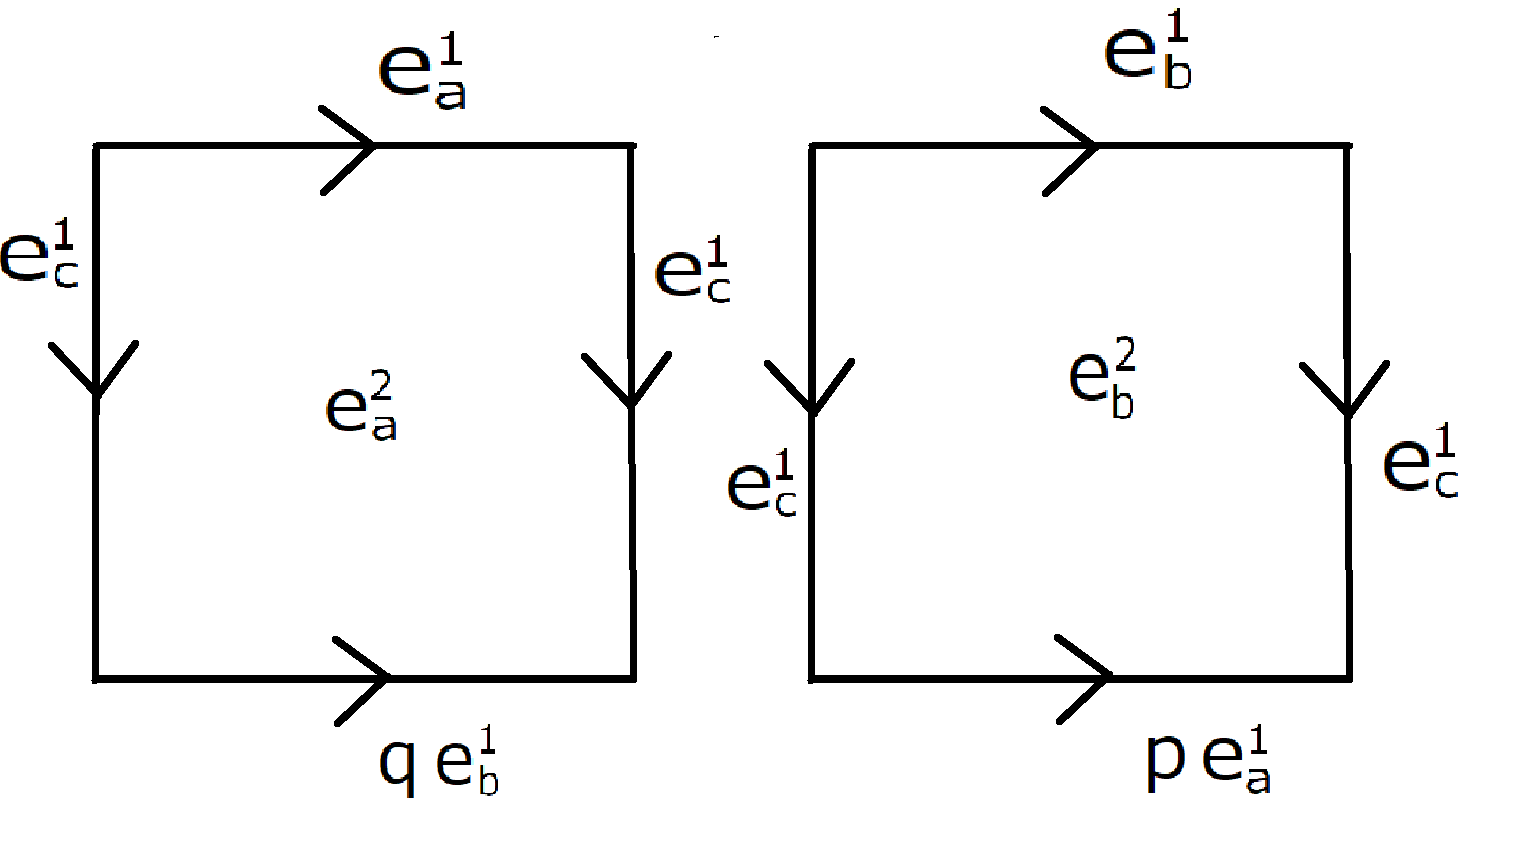
\includegraphics[width=5cm]{H31expert05_02.png}
\end{center}

のような状況になっているので
\[
\del(e_a^2) = e_a^1 - qe_b^1 \quad \del(e_b^2) = e_b^1 - pe_a^1
\]
である。したがって$\del$は次の行列
\[
\del = \pmat{
1 & -p \\
-q & 1 \\
0 & 0
}
\]
で表される写像である。この行列の階数は$pq =1$のとき$1$でそうでないとき$2$である。よって$pq = 1$のとき
\begin{align*}
  H_1(Y) &= \Z^3 / \Im \del \\
  &= \Z^2 \\
  H_2(Y) &= \Ker \del \\
  &= \Z
\end{align*}
である。$pq \neq 1$ならば
\begin{align*}
  H_1(Y) &= \Z^3 / \Im \del \\
  &= (a \Z \oplus  b \Z \oplus c \Z)  / (a - qb, b - pa) \\
  &= (a \Z \oplus  b \Z )  / ( (1-pq)a, b - pa) \oplus c \Z \\
  &= \Z / (1-pq)\Z \oplus \Z \\
  H_2(Y) &= \ker \del \\
  &= 0
\end{align*}
である。以上により求めるホモロジーは、$pq = 1$のとき
\[
H_i(Y) = \begin{cases}
\Z &(i=0,2) \\
\Z^2 &(i=1) \\
0 &(\text{otherwise})
\end{cases}
\]
であり、$pq \neq 1$のとき
\[
H_i(Y) = \begin{cases}
\Z &(i=0) \\
\Z / (pq-1)\Z \oplus \Z &(i=1) \\
0 &(\text{otherwise})
\end{cases}
\]
\end{sol}
